\documentclass{article}
\usepackage[utf8]{inputenc}
\usepackage{t1enc}
\usepackage{geometry}
 \geometry{
 a4paper,
 total={210mm,297mm},
 left=20mm,
 right=20mm,
 top=20mm,
 bottom=20mm,
 }
\usepackage{amsmath}
\usepackage{amssymb}
\frenchspacing
\usepackage{fancyhdr}
\pagestyle{fancy}
\lhead{Urbán János tanár úr feladatsorai}
\chead{C08/1/07}
\rhead{Halmazok}
\lfoot{}
\cfoot{\thepage}
\rfoot{}

\usepackage{enumitem}
\usepackage{multicol}
\usepackage{calc}
\newenvironment{abc}{\begin{enumerate}[label=\textit{\alph*})]}{\end{enumerate}}
\newenvironment{abc2}{\begin{enumerate}[label=\textit{\alph*})]\begin{multicols}{2}}{\end{multicols}\end{enumerate}}
\newenvironment{abc3}{\begin{enumerate}[label=\textit{\alph*})]\begin{multicols}{3}}{\end{multicols}\end{enumerate}}
\newenvironment{abc4}{\begin{enumerate}[label=\textit{\alph*})]\begin{multicols}{4}}{\end{multicols}\end{enumerate}}
\newenvironment{abcn}[1]{\begin{enumerate}[label=\textit{\alph*})]\begin{multicols}{#1}}{\end{multicols}\end{enumerate}}
\setlist[enumerate,1]{listparindent=\labelwidth+\labelsep}

\usepackage{pgf,tikz}

\newcommand{\degre}{\ensuremath{^\circ}}
\newcommand{\tg}{\mathop{\mathrm{tg}}\nolimits}
\newcommand{\ctg}{\mathop{\mathrm{ctg}}\nolimits}
\newcommand{\arc}{\mathop{\mathrm{arc}}\nolimits}
\renewcommand{\arcsin}{\arc\sin}
\renewcommand{\arccos}{\arc\cos}
\newcommand{\arctg}{\arc\tg}
\newcommand{\arcctg}{\arc\ctg}

\parskip 8pt
\begin{document}

\section*{Halmazok}

\subsection*{2008.11.20.}
\begin{enumerate}
\item Legyen a $H{=}\{1,2,3,4\ldots,19,20\}$ alaphalmaz három részhalmaza:\\
$A=${\{}a $20$-nál nem nagyobb pozitív páros számok{\}},\\
$B=${\{}$5k|$ $k{\in}N$, $1{\le}k{\le}4${\}},\\
$C={\{}1,2,3,4,\ldots,9,10{\}}$.\\
Határozzuk meg a következő halmazokat:
$\overline{A{\cup}B}$, $\overline{B{\cap}C}$, $\overline{A{\cup}B{\cup}C}$, $\overline{C{\setminus}A}$, $\overline{(A{\cap}B){\cup}C}$.

\item Adott $H$ alaphalmaz és az $A, B, C$ részhalmazai.
Az ábrán $(1),(2),\ldots,(8)$ jelöli az egyes tartományokat.

\begin{center}
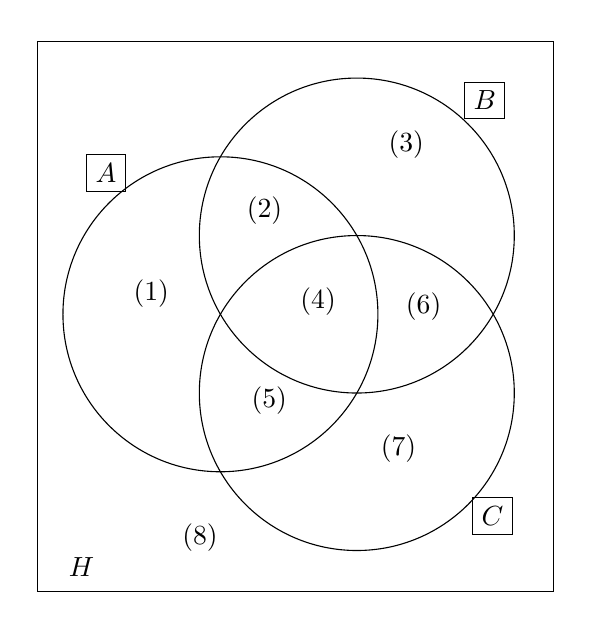
\begin{tikzpicture}[x=1.0cm,y=1.0cm]
\clip(-4.18,-0.72) rectangle (2.64,6.64);
\draw(-1.7320508075688772,3.) circle (2.cm);
\draw(0.,4.) circle (2.cm);
\draw(0.,2.) circle (2.cm);
\draw (-4.06,6.46)-- (2.5,6.46);
\draw (2.5,6.46)-- (2.5,-0.52);
\draw (2.5,-0.52)-- (-4.06,-0.52);
\draw (-4.06,-0.52)-- (-4.06,6.46);
\draw (-3.78,0.04) node[anchor=north west] {$H$};
\draw (-2.96,3.56) node[anchor=north west] {$(1)$};
\draw (-1.52,4.62) node[anchor=north west] {$(2)$};
\draw (0.28,5.46) node[anchor=north west] {$(3)$};
\draw (-0.84,3.46) node[anchor=north west] {$(4)$};
\draw (-1.46,2.2) node[anchor=north west] {$(5)$};
\draw (0.5,3.4) node[anchor=north west] {$(6)$};
\draw (0.18,1.6) node[anchor=north west] {$(7)$};
\draw (-2.34,0.46) node[anchor=north west] {$(8)$};
\draw (-3.56,5.16) node[anchor=north west] {\fbox{$A$}};
\draw (1.24,6.08) node[anchor=north west] {\fbox{$B$}};
\draw (1.34,0.8) node[anchor=north west] {\fbox{$C$}};
\end{tikzpicture}
\end{center}

\noindent Mely tartományokkal állnak a következő halmazok:
$(A{\cup}B){\cap}C$; $A{\cup}(B{\cap}C)$; $(A{\cap}B){\cup}C)$; $A{\cup}(B{\setminus}C)$;
$(B{\setminus}C){\cup}A$; $(B{\setminus}C){\cap}A$; $B{\setminus}(C{\cap}A)$; $B{\setminus}(C{\cup}A)$?

\item Az előző ábrán jelölt tartományok közül melyekből állnak a következő halmazok:
$\overline{A{\cup}B}$, $\overline{B{\cap}C}$, $\overline{C{\setminus}A}$, $\overline{(A{\setminus}B){\setminus}C}$, $\overline{(A{\cup}B){\cap}C}$, $\overline{A{\cap}(B{\cup}C)}$?

\item Ha $A{\setminus}B{=}{\varnothing}$, akkor mivel egyenlő 
$A{\cup}B$, $A{\cap}B$, $B{\setminus}A$?
\end{enumerate}


\subsection*{2008.11.25.}
\underline{Definíció:} $A{\subseteq}B$ ($A$ részhalmaza $B$-nek),
ha $x{\in}A \Rightarrow x{\in}B$.
\begin{enumerate}
\item Igazoljuk a következőket:
\begin{abc2}
\item $A{\subseteq}B$ és $B{\subseteq}A \Rightarrow A{=}B$;
\item $A{\subseteq}B$ és $B{\subseteq}C \Rightarrow A{\subseteq}C$.
\end{abc2}

\item Igazoljuk, hogy ha $A{\subseteq}B$, akkor $A{\cup}B=B$ és $A{\cap}B{=}A$,

\item Legyenek $A$ és $B$ véges halmazok ($|A|$ jelöli $A$ elemeinek számát). Igazoljuk:
\begin{abc2}
\item $|A{\cup}B|\le|A|+|B|$;
\item $|A{\cap}B|\le{\frac{|A|+|B|}{2}}$.
\end{abc2}

\item Adjunk példát olyan $A$, $B$ és $C$ halmazra, hogy teljesüljenek a következő feltételek:\\
$|A|{=}|B|{=}|C|{=}2$, $|A{\cap}B{\cap}C{=}1$ és $A{\not=}B$, $B{\not=}C$.

\item Adjunk meg három olyan kételemű halmazt, melyeknek páronként vett közös része nem üres, de a három halmaz része üres.

\item Az $A$ és $B$ halmazokról tudjuk, hogy 
$A{\cup}B{=}\{1,2,3,4,5,6\}$, $A{\setminus}B{=}\{2,4,6\}$, $A{\cap}B{=}\{1,3\}$.\\
Mik lehetnek $A$ elemei és $B$ elemei?
\end{enumerate}


\subsection*{2008.11.27.}
\begin{enumerate}

\item Definíció: $A{\bigtriangleup}B{=}(A{\setminus}B){\cup}(B{\setminus}A)$;
igazoljuk, hogy
\begin{abc2}
\item $A{\bigtriangleup}B{=}B{\bigtriangleup}A$;
\item $|A{\bigtriangleup}B|{=}|A|+|B|-2|A{\cap}B|$.
\end{abc2}

\item Igazoljuk a következő azonosságokat:
\begin{abc2}
\item $(A{\bigtriangleup}B){\bigtriangleup}C{=}A{\bigtriangleup}(B{\bigtriangleup}C)$;
\item $A{\bigtriangleup}(A{\bigtriangleup}B){=}B$;
\item $(A{\bigtriangleup}B){\cap}C{=}(A{\cap}C){\bigtriangleup}(B{\cap}C)$.
\end{abc2}

\item Az $A$, $B$, $C$ halmazokról tudjuk, hogy $A{\setminus}B{=}\{4,6,8\}$, $B{\setminus}C{=}\{2,5,9,10\}$, $C{\setminus}A{=}\{3,7,11\}$, $A{\cap}B{\cap}C{=}
\{1\}$, $A{\cup}B{=}\{1,2,3,4,5,6,8,9,10,11\}$, $C{\cup}A{=}\{1,2,3,4,5,6,7,8,9,11\}$, és $|C|{=}5$.
\\Határozzuk meg az $A$, $B$, $C$ halmazokat.

\item Az $A$ és $B$ halmazokról tudjuk, hogy $|A|{=}5$, $|B|{=}8$, $|A{\setminus}B|{=}3$.
Számítsuk ki $|A{\cup}B|$ és $|A{\cap}B|$ értékét.

\item Ha $A{=}\{100$-nál nem nagyobb pozitív négyzetszámok$\}$,
 $B{=}\{$a $9$-cel osztható legfeljebb kétjegyű pozitív egészek$\}$,
 akkor számítsuk ki $|A|$, $|B|$,  $|A{\setminus}B|$, $|B{\setminus}A|$,
 $|A{\cup}B|$, $|A{\cap}B|$ értékét.
\end{enumerate}

\subsection*{2008.12.01.}
\begin{enumerate}
\item Tudjuk, hogy $|A|{=}8$, $|B|{=}11$. Mekkora 
lehet $|A{\cap}B|$, $|A{\cup}B|$, $|A|{\setminus}|B|$,
$|A{\cap}B|$ ?

\item Tudjuk, hogy $|A{\cup}B|{=}6$, $|A{\setminus}B|{=}3$,
$|A{\cap}B|{=}2$. Mekkora lehet $|A|$ és $|B|$ ?

\item Az $A$, $B$, $C$ halmazokról tudjuk, hogy $|A{\setminus}B|{=}5$, $|B{\setminus}C|{=}5$, $|C{\setminus}A|{=}4$, 
$|A{\cap}B{\cap}C|{=}1$, $|A{\cup}B|{=}13$, $|A{\cup}C|{=}12$, $|C|=7$.
 Mennyi lehet $|A|$ és $|B|$?

\item Tudjuk, hogy $|A{\cup}B|{=}7$, $|A{\cup}C|{=}7$, $|B{\cup}C|{=}6$.
 Mennyi az a legkisebb és legnagyobb érték, amit $|A{\cup}B{\cup}C|$ felvehet?

\item Tudjuk, hogy $|A|{=}7$, $|B|{=}8$, $|C|{=}9$, $(A{\cap}B{\cap}C){=}3$.
 Mennyi az a legkisebb és legnagyobb érték, amit $|A{\cup}B{\cup}C|$ felvehet?

\item Adjunk meg 4 olyan halmazt, amelyekre teljesül az alábbi feltételek mindegyike:
\\(1) bármely kettőnek van közös eleme;
\\(2) bármely három halmaz metszete üres halmaz;
\\(3) a halmazok elemszáma egyenlő;
\\(4) a halmazok elemszáma a lehető legkisebb.
\end{enumerate}

\subsection*{2008.12.02}
\underline{Definíció}: $A{\times}B{=}\{(a;b)|$ $a{\in}A$, $b{\in}B\}$ \\
Például: $A{=}\{1,2\}$, $B{=}\{3,4\}$ $\Rightarrow$ $A{\times}B{=}\{(1;3),(1;4),(2;3),(2;4)$.

\begin{enumerate}
\item Legyen $A{=}B{=}\{0,1,2\}$ adjuk meg az $A{\times}B$ halmazt.

\item $A{=}\{1,2,3\}$, $B{=}\{2,3,4\}$. Hány eleme van a következő halmazoknak $(A{\setminus}B){\times}(B{\setminus}A)$; $(A{\cup}B){\times}(B{\cap}A)$?

\item Legyen $A$ a $100$-nál nem nagyobb pozitív halmazok száma, B pedig a $200$-nál nem nagyobb pozitív számok halmaza. Mennyi eleme van  az $(A{\times}B){\setminus}(B{\times}A)$ és a $(B{\times}A){\setminus}(A{\times}B)$ halmaznak?

\item $A$ és $B$ olyan véges halmazok, amelyre teljesül, hogy $|A{\times}B|{=}100$. Határozzuk meg $|A{\cup}B|$ és $|A{\cap}B|$ minimumát és maximumát.

\item Legyen $A$, $B$, $C$ amelyekre $|A|{=}|B|{=}|C|{=}5$ $|A{\cup}B{\cup}C|{=}1$. Határozzuk meg $|A{\cup}B{\cup}C|$ minimális és maximális értékét.

\item  Igazoljuk: $A{\setminus}(B{\cup}C){=}(A{\setminus}B){\cap}(A{\setminus}C)$ és $A{\setminus}(B{\cap}C){=}(A{\setminus}B){\cup}(A{\setminus}C)$
\end{enumerate}

\subsection*{2008.12.03}
\begin{enumerate}
\item Legyen $A{=}\{3$-mal osztható kétjegyű számok\}, $B{=}\{7$-tel osztható kétjegyű számok\}. $|A{\cup}B|{=}$? és $|A{\cap}B|{=}$?

\item $A{=}\{1,2\}$, $B{=}\{1,2,3,4\}$, Írjuk fel az $(A{\times}A){\cap}(B{\times}B)$ halmaz elemeit.

\item $A{=}\{1,2,3,4\}$, $A{\cup}B{=}A$, $A{\cap}B{=}B$ mi lehet a $B$ halmaz?

\item Legyen $H{=}{\frac{2}{1}, \frac{4}{3}, \frac{6}{5}, {\ldots}, \frac{1002}{1001}}$. Hány olyan $x$ eleme van a $H$ halmaznak amelyre, $|x-1|<0,1$?

\item Egy osztály létszáma $30$. Az osztályban $3$ nyelvet tanulnak, angolt, németet és franciát és minden diák legalább egy nyelvet tanul. Angolul $14$-en, németül $15$-en, franciául $5$-en tanulnak. Pontosan két  nyelvet $6$ diák tanul. Hányan tanulják mindhárom nyelvet?

\item $|A|{=}7$, $|B|{=}8$, $|C|{=}9$, $|A{\cap}B{\cap}C|{=}3$,  ?${\le} |A{\cup}B{\cup}C|{\le}$?

\item ($*$) Adjunk meg három olyan halmazt, amelyeknek végtelen sok eleme van, bármely kettő is végtelen halmaz, a három halmaz közös része üres.
\end{enumerate}
\end{document}
